% chap3.tex

\begingroup
    \fontsize{10pt}{12pt}\selectfont
    \begin{verbatim}  
         
    \end{verbatim}  
\endgroup

\chapter{Visibility Driven Transfer functions}\label{chap:ch4_abbr}

\section{Motivation}

Medical imaging has given radiologists an ability that photography was not able to provide, it lets them see inside the human body. With the advent of 3D visualization systems, these images can be put together into crisp and impressive renderings of the human body from a variety of perspectives that were only dreamt of before, revolutionizing clinical practice.

Light transport models soon emerged to allow light interactions that, although not realistic in the physical sense, proved to be more effective for understanding the complex relationships among the anatomical structures. For instance, bone could be made semi-transparent to provide visibility of brain tissue. Skin could be removed altogether from an image to show only muscle or internal organs. However, soon it
became evident that simply rendering these images in their raw form was no longer effective and the clear visualization of internal structures remains elusive.

The depiction of internal parts in the context of the enclosing space is a difficult problem that has occupied the mind of artists, illustrators and visualization practitioners. Despite the advances made in computer graphics for simulating the light transport in semi-transparent media, the problem of visualizing internal objects is no longer a rendering problem, but that of classification. Medical imaging technology obtains representations of anatomical structures via indirect ways, such as the response of tissue to X-rays or the alignment of electrons in a magnetic field. Therefore, the absence of semantic information prevents visualization practitioners from clearly marking up the regions that must be visualized. Without access to those regions, exploration becomes tedious and time-consuming. The predominant approach has been the use of transfer functions, or opacity mappings, which assign transparency and color properties to different intervals in the data. This method, however, does not guarantee visibility of internal structures or structures of interest in the volume. There is need to incorporate a measure for visibility, which gives contribution of each volume element in making of final image. In this chapter, visualization techniques to obtain clear views of internal features in 3D volume data are discussed along with visibility metric.

\section{Related Work}

With the fast growth in computational power of graphics hardware, it has recently become possible to manipulate 3D volume data in fashions that were only possible for surface meshes and CAD models, where semantic information is often explicit and readily available. When volume data are understood as explorable objects, it can be disassembled into parts that can be decomposed in numerous ways. One of the foremost ideas that were explored in this direction were cutaways, where certain parts can be removed to uncover hidden parts of the 3D volume~\cite{c}. Exploded views extend this idea to reveal the relationships among the internal parts of a complex volume~\cite{b}, as shown in figure 3.1.

\begin{figure}[!h]
\centering
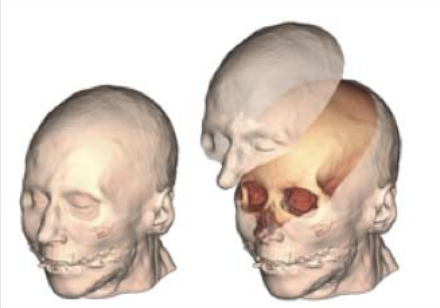
\includegraphics[width=220pt]{Images/cut-away.png}
\caption{\label{fig:ray_cast1.jpg} Cutaway of the skin of a CT data set~\cite{b}.}
\end{figure}

Another strategy is to assign material properties to different regions or layers of a volume and simulate the physical response to the deformation and cutting of such regions~\cite{d}. Figure 3.2, for example, shows the result of simulating a peel away on a CT scan of a piggy bank to reveal a number of coins in its interior.

\begin{figure}[!h]
\centering
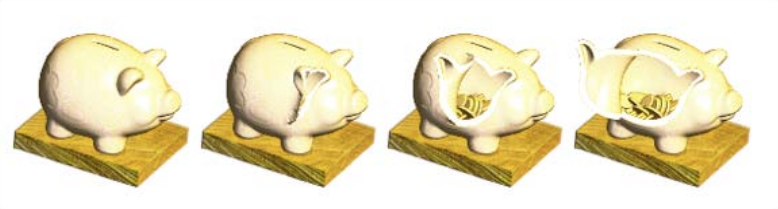
\includegraphics[width=250pt]{Images/vol-peeling.png}
\caption{\label{fig:ray_cast1.jpg} Volume peeling of a CT scan of a piggy bank~\cite{peel}.}
\end{figure}

Rigid and deformable cuts, although effective for visualizing the internal structures, work under the premise that the internal and external layers are clearly separated. In a more general sense, this separation is not easy to come by, and, in most cases, there is a degree of uncertainty. For this reason, the effective visualization of internal structure must rely on robust classification.

The main challenge when attempting to see the internal features remains that of classification. An effective visualization must first decide what regions it must preserve, and what regions are unimportant. However, volume data seldom contain any semantics about the captured structures. Acquisition technology outputs a series of images with intensity values, while simulations of 3D phenomena sample a continuous scalar or vector field in a grid. Therefore, traditional classification systems, found in off-the-shelf visualization systems, only consider a single dimension for classification, without regards of the spatial characteristics or the semantics of the data.

In an attempt to extract semantic information, one may analyze the spatial properties of the data, such as the location of boundaries~\cite{e}, regions of high curvature~\cite{a}, or shape~\cite{f}. In most of these cases, these properties are just approximations of the local distribution of data in a small neighborhood. Size, for example, can be measured as the extents of regions of certain homogeneity. Regions of a certain material, such as brain, that occupy a large volume, have different properties than those regions, such as skull and
skin, that are relatively thin.

These observations have enabled us to construct classification based on size, and assign opacity based on the relative thickness of features. A particular example is the visualization of brain MRI, where the data is comprised of a series of thin layers (i.e, skin, skull and tissue) surrounding a large region, the brain, of a certain material. Exploiting these properties lets us minimize the effects of occluding tissue, such as skin, to reveal the brain tissue clearly, as shown in figure 3.3.

\begin{figure}[!h]
\centering
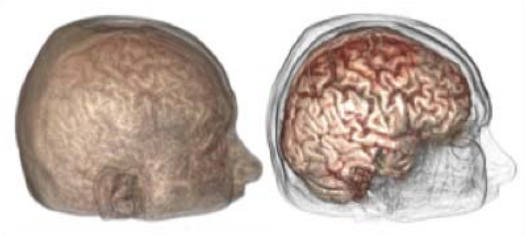
\includegraphics[width=250pt]{Images/size-tf.png}
\caption{\label{fig:ray_cast1.jpg} Size-based transfer function to visualize the brain. On the left is the original rendering, where brain is obscured by the skin~\cite{a}.}
\end{figure}

\section{Visibility histogram}

\subsection{Visibility} 

One of the limitations of contemporary visualization systems is the inability to quantify how visible a feature of interest is. To be more effective, along with traditional transfer function design, visualization systems must also incorporate a measure of visibility. 

Visibility Metric, as defined in~\cite{vdtf}, attemps to measure the impact of individual samples on the image generated by a volumetric object. It is measured as the contribution of a structure of interest to the final image. Here, visibility can be used to quantify the quality of transfer function and ease their design towards more meaningful and efficient visualization. Transfer functions generated with this approach are called as visibility driven tranfser functions.

This process measures visibility of all structures in a volume to arrive at a good transfer function. In general, a visibility-driven transfer function is constructed in such a way that it attempts to guarantee the visibility of all structures of a volume and at the same time maximizes the visibility of structure of interest, in particular, of those features lying at the interior of a data set. 

\subsection{Visibility Histogram}

The contribution of a sample in the volume to final image is referred to as visibility of that sample. 

\begin{equation}
\alpha (s) \; = \; 1 \; - \; e^{\int^{D}_{s} \tau(t) dt \; }  
\end{equation}   


where $ \tau(t) $ is the attenuation coefficient of a sample, usually represented as an opacity transfer function $\mathcal{O}$ which is defined by user. Visibility also depends on viewpoint as accumulated opacity in front of the sample may differ at different viewpoints. 

A visibility histogram is a representation of distribution of the visibility metric in relation to the domain values of the volume. Samples are weighted by visibility and added into bins that partition the range of values in the scalar field. 

\begin{equation}
VH(x) =  \mathcal{O} (x) \int_{s \epsilon \omega} \delta(s, x) (1 \; - \; \alpha(s) ) ds 
\end{equation}
where, $ \delta(s, x) $ is a function.


\begin{equation}
    \delta(s, x)=\left\{
                \begin{array}{ll}
                  1  \;\;\;\;\;\;\;    V(s) = x\\
                  0  \;\;\;\;\;\;\;    Otherwise\\
                \end{array}
              \right.
\end{equation}

Hence, for all sample values x in the volume.

\begin{equation}
VH[x] = VH[x] + ( 1 - AccumulatedOpacity ) Opacity(x) 
\end{equation}

\begin{figure}
\centering
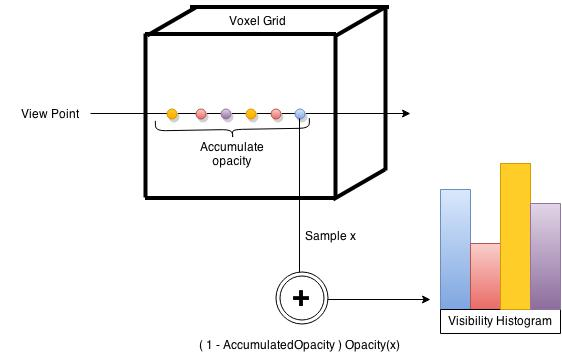
\includegraphics[width=250pt]{Images/VHistogram.jpg}
\caption{\label{fig:ray_cast1.jpg} Visibility histogram computation using Raycasting.}
\end{figure}


\subsection{Influence of the Transfer Function}

Visibility histograms are transfer function dependent. A visibility histogram depicts the visibility distribution for a given data set only
with respect to a certain transfer function. Every time the alpha transfer function changes, the visibility histogram has to be recomputed. Figure 3.5 shows how different transfer functions applied to the same dataset can lead to different visibility distributions. \\

\begin{figure}
\centering
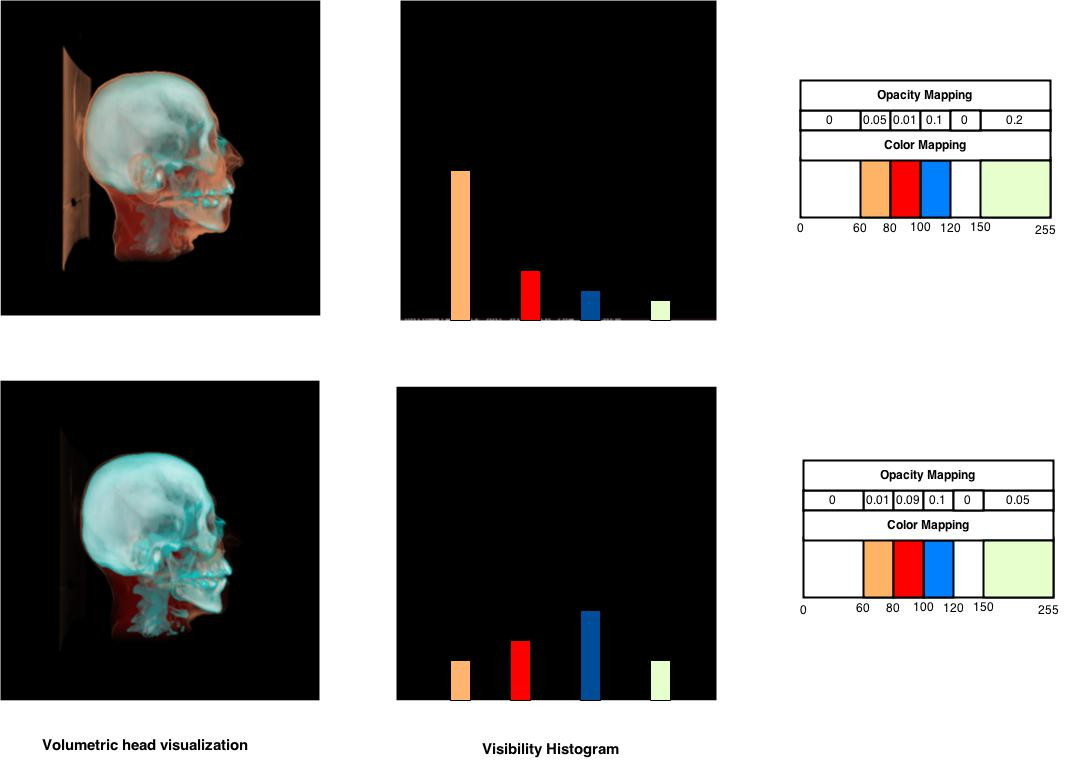
\includegraphics[width=450pt]{Images/tf_influence.jpg}
\caption{ Illustration of influence of opacity mapping on the visibility histogram when viewing direction and sampling stepsize is constant. }
\end{figure}

\subsection{Influence of the Viewing Direction}

A visibility histogram for a particular dataset is dependent on the direction from which the dataset is looked at, i.e. the direction of the viewing rays which traverse the data set. On rotating the dataset, the sample points that are encountered along the viewing rays change, causing a change in the visibility distribution, as shown in figure 3.6. \\

\begin{figure}
\centering
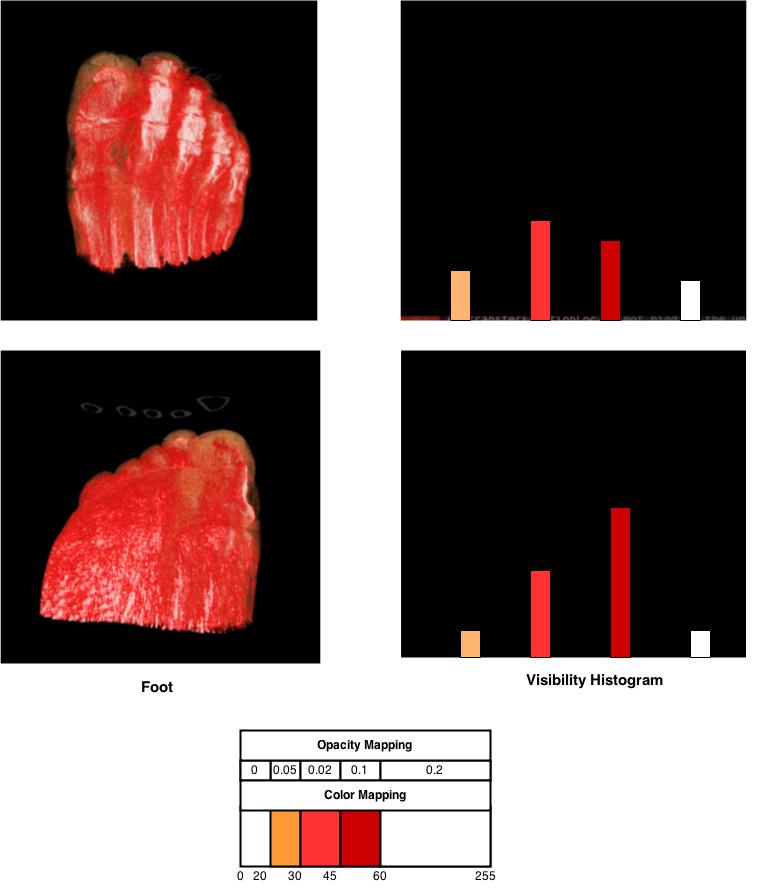
\includegraphics[width=450pt]{Images/tf_view_influence.jpg}
\caption{ Illustration of influence of viewing direction on visibility histogram when transfer function and sampling stepsize is constant. }
\end{figure}


\section{Role Of Raycasting In Computing Visibility Histogram}

As discussed in previous chapter, section 2.3, we know that basic idea behind volume ray casting is to shoot viewing rays through the data
volume for every pixel in the image plane, and samples are taken at evenly spaced points (see figure 2.5) and blended together using the front-to-back compositing scheme defined by equation 2.5 and 2.6 to calculate the intensity value for the pixel in the image plane from which the ray originated.

\newpage
\section{Transfer Function Design}

\subsection{Manually Generated Transfer Functions}

\begin{figure}
\centering
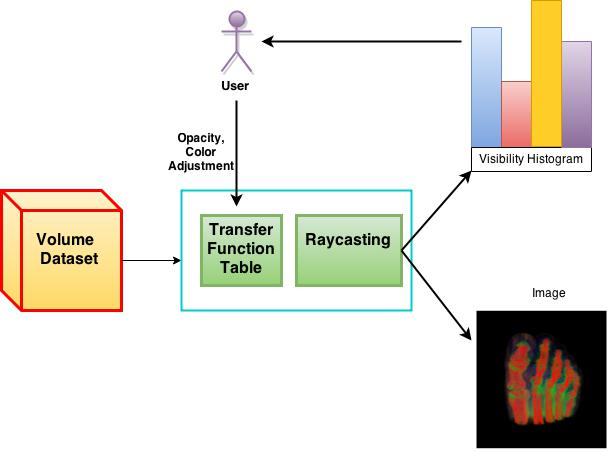
\includegraphics[width=350pt]{Images/VH_pipeline.jpg}
\caption{\label{fig:ray_cast1.jpg} Transfer function design using visibility histogram.}
\end{figure}

Trial and error is used commonly for finding an appropriate transfer function for a certain dataset. This approach is easy to handle, but can be very time consuming. The transfer function is typically generated by the user. Then, the dataset is rendered with the specified transfer function. If the resulting image does not meet the user\'s expectations, the transfer function is modified. This keeps untill user's expectation is met. The problem with this approach is that the user has lots of possibilities for generating and modifying transfer functions, and it might take a huge number of steps to find an appropriate one. 

To address this issue, visibity histogram provides visual cues on contribution of samples in making of the final image. The visibility histogram itself is important as a visual aid. 

As shown in the figure 3.7, the volumetic data is rendered using volume raycasting with the transfer function defined by user to generate final image and it's corresponding visibility histogram. The visibility histogram, which is generally plotted as a graph, provides immediate feedback to user regarding contributions of volume elements in the final image. The Visibility histogram helps find occulsion patterns on the data, as shown in figure 3.8, which helps in opacity modulation in a intuitive fashion to generate user desired results. Since, feedback mechanism is interactive, opacity modulation is easier and desired images are generated quickly.    


\begin{figure}
\centering
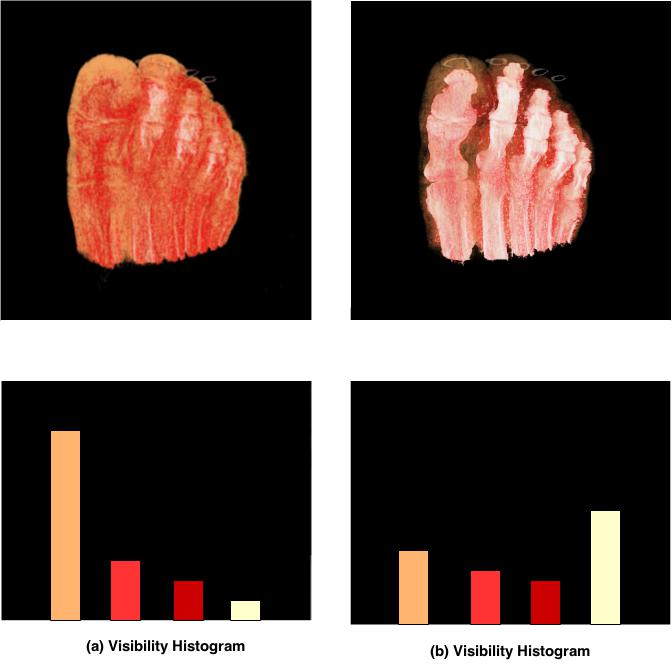
\includegraphics[width=350pt]{Images/occlusion.jpg}
\caption{\label{fig:ray_cast1.jpg} Visibility histogram depicting occlusion signature of a foot dataset. (a) The signature on the histogram reveals presence of a strong occluder. (b) The signature of this histogram reveals no presence is a strong occluder. }
\end{figure}


\subsection{Semi-automatic Transfer Functions Design}

A further goal is to automate design of transfer functions that would result in improved visibility of the regions of interest. This has been  formulated as an energy minimization problem~\cite{vdtf}. The following energy components, designed to highlight certain desired aspects of the transfer function are:

\begin{itemize}
\item User-satisfaction: To ensure user-satisfaction, we minimize the mismatch between the computed opacity function and the original one defined by the user.
\item Visibility: The second component is used to maximize the visibility of a given sample.
\item Constraint: These constraints are used to control the minimum and maximum values opacities of value intervals in the final opacity function. 
\end{itemize}
 
In the thesis, we have not focused on semi-automatic transfer function design aspect. 

\section{Focus+Context Using Visibility Histograms}

A region of interest can be a range of voxel intensities, and this segmentation is achieved using transfer function. From section 3.3.2, we know that visibility histogram gives graphical cues on visibility of samples in making of the final image. Since range of voxel intensities define the ROI, visibility histogram can be used to find visibility of the ROI. Visibility histogram also reveals the occluding patterns, as illustrated in figure 3.8. Using the visual cues from the Visibility Histogram, the user can modulate opacities to set the focus on ROI. Tradeoff between visibility and spatial clarity can be handled, by adjusting opacities of regions surrounding the ROI untill it meets user requirement. \\

A region of interest can also be a volume, which is set of voxels within an 3D volume. Figure 3.9, illustrates volume ROI on volumetric head dataset, figure 3.9(a) shows original rendering and figure 3.9(b) shows volume ROI defined in the neck region, allowing the visualization of insides of the neck area.

\begin{figure}
\centering
\begin{subfigure}{0.6\textwidth}
  \centering
  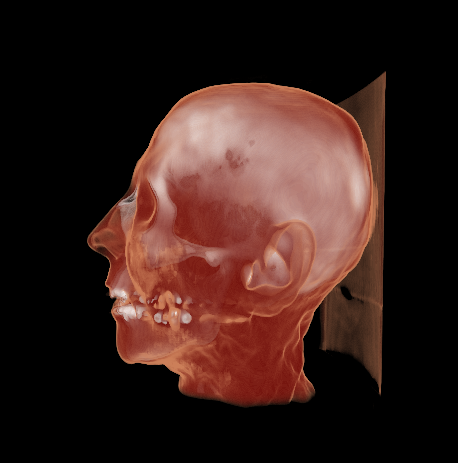
\includegraphics[width=0.9\linewidth]{Images/NON-VOI.png}
  \caption{Original }
  \label{fig:sub1}
\end{subfigure}
\begin{subfigure}{0.6\textwidth}
  \centering
  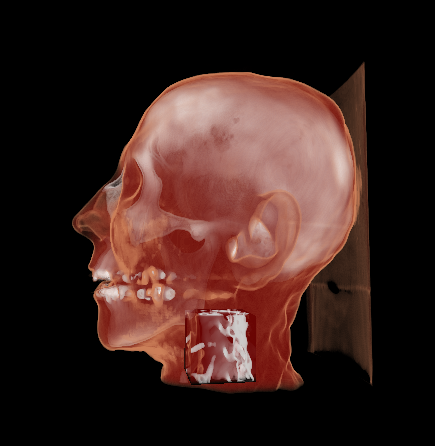
\includegraphics[width=0.9\linewidth]{Images/VOI.png}
  \caption{Volume-defined ROI}
  \label{fig:sub2}
\end{subfigure}
\label{fig:test}
\caption{Illustration of Volume-defined ROI}
\end{figure}


   

